\vspace*{1em}
\chapter{Các Phương Pháp Lặp Trong Đại Số Ma Trận}

\section{Các kỹ thuật lặp Jacobi và Gauss–Seide (The Jacobi and Gauss–Seidel Iterative Techniques)}

Trong phần này ta trình bày chi tiết hai phương pháp lặp cơ bản dùng để giải hệ tuyến tính
\[
A\mathbf{x}=\mathbf{b},\qquad A\in\mathbb{R}^{n\times n},\ \mathbf{b}\in\mathbb{R}^n,
\]
và sau đó đưa ra dạng tổng quát của các phương pháp lặp tuyến tính. Các phương pháp này là nền tảng
cho nhiều phương pháp lặp tiên tiến hơn (như SOR, CG, v.v.).

\subsection{Jacobi's Method}

\textbf{Phân rã ma trận.}
Ta phân rã ma trận $A$ theo
\[
A = D + L + U,
\]
trong đó $D$ là ma trận đường chéo gồm các $a_{ii}$, $L$ là ma trận tam giác dưới (phần dưới đường chéo, với dấu âm nếu muốn theo một dạng khác) và $U$ là ma trận tam giác trên, sao cho thường viết
\[
A = D - L - U
\]
khi muốn lấy $L$ và $U$ là các ma trận có dấu âm của các phần tử ngoài đường chéo.

\textbf{Dẫn xuất công thức Jacobi.}
Giải phương trình thứ $i$ trong $A\mathbf{x}=\mathbf{b}$ theo $x_i$:
\[
a_{ii} x_i = b_i - \sum_{\substack{j=1\\ j\ne i}}^{n} a_{ij} x_j,
\]
và do đó một công thức lặp thuần túy (không dùng phần tử vừa cập nhật) là
\[
x_i^{(k+1)} = \frac{1}{a_{ii}}\Big( b_i - \sum_{\substack{j=1\\ j\ne i}}^{n} a_{ij} x_j^{(k)}\Big),
\qquad i=1,\dots,n.
\]
Viết theo dạng vectơ, ta có dạng lặp
\[
\mathbf{x}^{(k+1)} = D^{-1}(\mathbf{b} - (L+U)\mathbf{x}^{(k)})
          = T_J \mathbf{x}^{(k)} + \mathbf{c}_J,
\]
với
\[
T_J = -D^{-1}(L+U),\qquad \mathbf{c}_J = D^{-1}\mathbf{b}.
\]

\textbf{Thuật toán Jacobi (tóm tắt).}
\begin{enumerate}
  \item Chọn một xấp xỉ khởi đầu $\mathbf{x}^{(0)}$.
  \item Với $k=0,1,2,\dots$ và với mỗi $i=1,\dots,n$ tính
    \[
    x_i^{(k+1)} = \frac{1}{a_{ii}}\Big( b_i - \sum_{j\ne i} a_{ij} x_j^{(k)}\Big).
    \]
  \item Dừng khi $\|\mathbf{x}^{(k+1)}-\mathbf{x}^{(k)}\|$ hoặc $\|A\mathbf{x}^{(k+1)}-\mathbf{b}\|$ nhỏ hơn một ngưỡng TOL.
\end{enumerate}

\textbf{Nhận xét về Jacobi.}
\begin{itemize}
  \item \textbf{Ưu điểm:} Rất dễ triển khai; mỗi bước cập nhật các thành phần độc lập dựa trên vòng trước → thuận lợi cho tính toán song song.
  \item \textbf{Nhược điểm:} Thường hội tụ chậm; cần điều kiện về cấu trúc ma trận để đảm bảo hội tụ.
\end{itemize}

\subsection{Jacobi Iterative — Điều kiện hội tụ}

\textbf{Ma trận lặp và spectral radius.}
Dạng tổng quát lặp tuyến tính là
\[
\mathbf{x}^{(k+1)} = T\mathbf{x}^{(k)} + \mathbf{c}.
\]
Một điều kiện cần và đủ để lặp hội tụ cho mọi xấp xỉ ban đầu là
\[
\rho(T) < 1,
\]
trong đó $\rho(T)$ là bán kính phổ của $T$ (max tuyệt đối các trị riêng).

\paragraph{Điều kiện đủ tiêu biểu.}
Một điều kiện dễ kiểm tra và thường dùng là \textbf{chéo trội nghiêm ngặt theo hàng}:
\[
|a_{ii}| > \sum_{j\ne i} |a_{ij}|,\qquad i=1,\dots,n.
\]
Nếu $A$ chéo trội theo hàng, thì cả ma trận Jacobi $T_J$ lẫn ma trận Gauss--Seidel $T_{GS}$ đều có $\rho<1$ và do đó hội tụ.

\textbf{Chuẩn và bất đẳng thức nghiệm.}
Dựa vào bất đẳng thức về chuẩn, nếu tồn tại một chuẩn ma trận $\|\cdot\|$ sao cho $\|T\|<1$ thì lặp hội tụ. Thực tế hay dùng chuẩn $\infty$ hoặc $1$ để kiểm tra chéo trội:
\[
\|T_J\|_\infty = \max_i \sum_{j\ne i} \frac{|a_{ij}|}{|a_{ii}|}.
\]

\subsection{The Gauss--Seidel Method}

\textbf{Ý tưởng.}
Gauss--Seidel tận dụng ngay các thành phần vừa được cập nhật trong cùng một vòng lặp để tính phần tử tiếp theo. Cách viết trực tiếp:
\[
x_i^{(k+1)} = \frac{1}{a_{ii}} \Big( b_i - \sum_{j=1}^{i-1} a_{ij} x_j^{(k+1)} - \sum_{j=i+1}^{n} a_{ij} x_j^{(k)}\Big),
\quad i=1,\dots,n.
\]

\textbf{Dạng ma trận lặp.}
Tách $A=D-L-U$ (chú ý dấu) thì
\[
(D-L)\mathbf{x}^{(k+1)} = U \mathbf{x}^{(k)} + \mathbf{b},
\]
và do đó
\[
\mathbf{x}^{(k+1)} = (D-L)^{-1} U \mathbf{x}^{(k)} + (D-L)^{-1}\mathbf{b},
\]
với ma trận lặp
\[
T_{GS} = (D-L)^{-1} U,\qquad \mathbf{c}_{GS} = (D-L)^{-1}\mathbf{b}.
\]

\textbf{Thuật toán Gauss--Seidel (tóm tắt).}
\begin{enumerate}
  \item Chọn xấp xỉ khởi đầu $\mathbf{x}^{(0)}$.
  \item Với $k=0,1,2,\dots$:
    \begin{itemize}
      \item Lần lượt cho $i=1,\dots,n$ tính
        \[
        x_i^{(k+1)} = \frac{1}{a_{ii}} \Big( b_i - \sum_{j=1}^{i-1} a_{ij} x_j^{(k+1)} - \sum_{j=i+1}^{n} a_{ij} x_j^{(k)}\Big).
        \]
    \end{itemize}
  \item Dừng khi đạt điều kiện dừng.
\end{enumerate}

\textbf{Nhận xét về Gauss--Seidel.}
\begin{itemize}
  \item \textbf{Ưu điểm:} Thường hội tụ nhanh hơn Jacobi; ít vòng lặp hơn để đạt độ chính xác tương đương.
  \item \textbf{Nhược điểm:} Khó song song hóa vì cập nhật tuần tự; mỗi vòng cần tính $(D-L)^{-1}u$ ẩn, nhưng thực tế thực hiện bằng công thức cập nhật trực tiếp nên không cần nghịch đảo rõ ràng.
\end{itemize}

\subsection{Gauss--Seidel Iterative — Điều kiện hội tụ}

\textbf{Các điều kiện tiêu biểu.}
\begin{itemize}
  \item Nếu $A$ là \textbf{chéo trội nghiêm ngặt theo hàng}, thì cả Jacobi và Gauss--Seidel hội tụ.
  \item Nếu $A$ là \textbf{đối xứng xác định dương} (SPD), Gauss--Seidel hội tụ (một phần có thể chứng minh dựa trên phân tích SPD và phương pháp năng lượng).
\end{itemize}

\textbf{So sánh ma trận lặp.}
Thường có quan hệ
\[
\rho(T_{GS}) \le \rho(T_J),
\]
vì Gauss--Seidel tận dụng nhiều thông tin hơn trong mỗi vòng lặp; do đó Gauss--Seidel thường hội tụ nhanh hơn (ít vòng hơn) so với Jacobi.

\subsection{General Iteration Methods (Dạng tổng quát của phương pháp lặp)}

\textbf{Tổng quát hóa.}
Một phương pháp lặp tuyến tính tổng quát có dạng
\[
\mathbf{x}^{(k+1)} = T\mathbf{x}^{(k)} + \mathbf{c},
\]
với $T$ được lựa chọn dựa trên phân rã $A=M-N$ sao cho
\[
M\mathbf{x}^{(k+1)} = N \mathbf{x}^{(k)} + \mathbf{b},
\]
và do đó
\[
\mathbf{x}^{(k+1)} = M^{-1}N \mathbf{x}^{(k)} + M^{-1}\mathbf{b},
\]
hay $T=M^{-1}N$. Các lựa chọn khác nhau của $M,N$ đưa ra các phương pháp khác nhau:
\begin{itemize}
  \item Jacobi: $M=D$, $N=-(L+U)$.
  \item Gauss--Seidel: $M=D-L$, $N=U$.
  \item SOR (sẽ trình bày ở 7.4): $M = \frac{1}{\omega}D - L$, $N = \frac{1-\omega}{\omega}D + U$.
\end{itemize}

\textbf{Tiêu chí chọn $M$.}
Muốn $M$ dễ giải (chẳng hạn tam giác hoặc đường chéo) để mỗi bước lặp rẻ chi phí, đồng thời $T=M^{-1}N$ có bán kính phổ nhỏ để hội tụ nhanh.

\textbf{Phân tích hội tụ.}
Để kiểm tra hội tụ, ta thường xét $\rho(T)$ hoặc một chuẩn ma trận $\|T\|$. Nếu $\rho(T)<1$ thì mọi xấp xỉ khởi đầu dẫn tới hội tụ; nếu $\rho(T)\ge1$ thì tối thiểu tồn tại xấp xỉ ban đầu khiến không hội tụ.

\textbf{Tốc độ hội tụ và lỗi.}
Nếu lặp hội tụ tuyến tính, tồn tại số $\mu\in(0,1)$ sao cho
\[
\|\mathbf{x}^{(k)}-\mathbf{x}\| \le C \mu^k
\]
với $\mu\approx\rho(T)$. Việc giảm $\rho(T)$ (qua chọn $M,N$ thích hợp hoặc qua tiền tiền xử lý/preconditioning) là mục tiêu chính của các phương pháp cải tiến.

\subsection{Ví dụ minh họa (cụ thể)}

\textbf{Hệ mẫu.} Xét hệ
\[
\begin{aligned}
10x_1 - x_2 + 2x_3 &= 6,\\
- x_1 + 11x_2 - x_3 + 3x_4 &= 25,\\
2x_1 - x_2 + 10x_3 - x_4 &= -11,\\
3x_2 - x_3 + 8x_4 &= 15.
\end{aligned}
\]
Ma trận là chéo trội nên cả Jacobi và Gauss--Seidel hội tụ.

\textbf{Jacobi (hai vòng lặp đầu).}
Với $\mathbf{x}^{(0)}=\mathbf{0}$,
\[
\begin{aligned}
x_1^{(1)} &= \tfrac{1}{10}(6 + 0 - 0) = 0.6,\\
x_2^{(1)} &= \tfrac{1}{11}(25 + 0 + 0 - 0) \approx 2.2727,\\
x_3^{(1)} &= \tfrac{1}{10}(-11 - 0 + 0 + 0) = -1.1,\\
x_4^{(1)} &= \tfrac{1}{8}(15 - 0 + 0) = 1.875.
\end{aligned}
\]
Dùng các giá trị này để tính vòng tiếp theo (mọi cập nhật dùng giá trị của vòng trước).

\textbf{Gauss--Seidel (hai vòng lặp đầu).}
Với $\mathbf{x}^{(0)}=\mathbf{0}$,
\[
\begin{aligned}
x_1^{(1)} &= 0.6,\\
x_2^{(1)} &= \tfrac{1}{11}(25 + x_1^{(1)} + 0 - 0) \approx \tfrac{1}{11}(25 + 0.6)=2.3273,\\
x_3^{(1)} &= \tfrac{1}{10}(-11 - 2x_1^{(1)} + x_2^{(1)} + 0)\approx -0.9575,\\
x_4^{(1)} &= \tfrac{1}{8}(15 - 3x_2^{(1)} + x_3^{(1)})\approx 1.8316.
\end{aligned}
\]
Ta thấy Gauss--Seidel sử dụng ngay $x_1^{(1)}$ khi tính $x_2^{(1)}$, do đó hội tụ nhanh hơn trong thực nghiệm.

\subsection{Kết luận}

\begin{itemize}
  \item \textbf{Jacobi} và \textbf{Gauss--Seidel} là hai phương pháp lặp cơ bản, dễ triển khai và phù hợp cho ma trận thưa.
  \item Kiểm tra hội tụ dựa trên \textbf{bán kính phổ} $\rho(T)$ hoặc điều kiện chéo trội.
  \item Dạng tổng quát $M\mathbf{x}^{(k+1)} = N\mathbf{x}^{(k)} + \mathbf{b}$ bao quát nhiều phương pháp; chọn $M$ sao cho dễ giải trong mỗi bước và làm giảm $\rho(M^{-1}N)$.
  \item Các phương pháp nâng cao (SOR, tiền xử lý, CG) phát triển trên nền tảng này để cải thiện tốc độ hội tụ và mở rộng vùng áp dụng.
\end{itemize}


\subsection*{Định nghĩa 7.23}
Giả sử \textbf(\( \tilde{x} \in \mathbb{R}^n \)) là một nghiệm xấp xỉ của \textbf{hệ phương trình tuyến tính} được xác định bởi Ax = b.
\textbf{Vectơ dư} (residual vector) của \( \tilde{x} \) đối với hệ này được định nghĩa là r = b - A\( \tilde{x} \). Khi \( \tilde{x} \) trùng với nghiệm chính xác của hệ, ta có \( r = 0 \).


\section{Các phương pháp lặp cải tiến trong giải hệ phương trình tuyến tính}

Chúng ta đã thấy trong Mục 7.3 rằng tốc độ hội tụ của một phương pháp lặp phụ thuộc vào bán kính phổ của ma trận liên quan đến phương pháp đó. Một cách để tăng tốc hội tụ là chọn phương pháp có ma trận với bán kính phổ nhỏ nhất. Trước khi trình bày quy trình chọn phương pháp như vậy, ta cần giới thiệu một cách đo mới cho biết mức độ sai khác giữa nghiệm xấp xỉ và nghiệm chính xác của hệ tuyến tính. Cách này sử dụng một vectơ được mô tả trong định nghĩa sau.

\subsection*{Định nghĩa 7.23}
Giả sử \textbf(\( \tilde{x} \in \mathbb{R}^n \)) là một nghiệm xấp xỉ của \textbf{hệ phương trình tuyến tính} được xác định bởi Ax = b.
\textbf{Vectơ dư} (residual vector) của \( \tilde{x} \) đối với hệ này được định nghĩa là r = b - A\( \tilde{x} \). Khi \( \tilde{x} \) trùng với nghiệm chính xác của hệ, ta có \( r = 0 \). Giả sử ta có:

\[
\mathbf{r}^{(k)} = \bigl(r^{(k)}_{1},\, r^{(k)}_{2},\, \ldots,\, r^{(k)}_{n}\bigr)^{t}.
\]

là \textbf{vectơ dư} của \textbf{phương pháp Gauss--Seidel}, tương ứng với \textbf{vectơ nghiệm xấp xỉ}

\[
\mathbf{x}^{(k)} = (x^{(k)}_1,\, x^{(k)}_2,\, \ldots,\, x^{(k)}_{i-1},\, x^{(k-1)}_i,\, \ldots,\, x^{(k-1)}_n)^{t}.
\]

Thành phần thứ \( m \) của vectơ \( r^{(k)} \) được cho bởi
\[
r^{(k)}_m = b_m - \sum_{j=1}^{i-1} a_{mj} x^{(k)}_j - \sum_{j=i}^{n} a_{mj} x^{(k-1)}_j, \tag{7.13}
\]
hay tương đương,
\[
r^{(k)}_m = b_m - \sum_{j=1}^{i-1} a_{mj} x^{(k)}_j - \sum_{j=i+1}^{n} a_{mj} x^{(k-1)}_j - a_{mi}x^{(k-1)}_i,
\]
với mỗi \( m = 1, 2, \ldots, n.\)

Đặc biệt, thành phần thứ \( i \) của \( r^{(k)} \) là
\[
r^{(k)}_i = b_i - \sum_{j=1}^{i-1} a_{ij}x^{(k)}_j - \sum_{j=i+1}^{n} a_{ij}x^{(k-1)}_j,
\]
do đó
\[
a_{ii}x^{(k-1)}_i + r^{(k)}_i = b_i - \sum_{j=1}^{i-1} a_{ij}x^{(k)}_j - \sum_{j=i+1}^{n} a_{ij}x^{(k-1)}_j. \tag{7.14}
\]

Nhắc lại rằng trong \textbf{phương pháp Gauss--Seidel}, \( x^{(k)}_i \) được chọn sao cho
\[
x^{(k)}_i = \frac{1}{a_{ii}}\left[b_i - \sum_{j=1}^{i-1} a_{ij}x^{(k)}_j - \sum_{j=i+1}^{n} a_{ij}x^{(k-1)}_j\right], \tag{7.15}
\]
vì vậy phương trình (7.14) có thể được viết lại thành
\[
a_{ii}x^{(k-1)}_i + r^{(k)}_i = a_{ii}x^{(k)}_i.
\]
Do đó, phương pháp Gauss--Seidel có thể được đặc trưng bởi điều kiện rằng \( x^{(k)}_i \) thỏa mãn
\[
x^{(k)}_i = x^{(k-1)}_i + \frac{r^{(k)}_i}{a_{ii}}. \tag{7.16}
\]

Ta có thể thiết lập thêm một mối liên hệ khác giữa các vectơ dư và kỹ thuật Gauss--Seidel. 
Xét vectơ dư \( r^{(k)}_{i+1} \) tương ứng với vectơ 
\(
x_{i+1}^{(k)} = (x^{(k)}_1,\, \ldots,\, x^{(k)}_i,\, x^{(k-1)}_{i+1},\, \ldots,\, x^{(k-1)}_n)^{t}.
\)
Theo công thức (7.13), thành phần thứ \( i+1 \) của \( r^{(k)} \) là
\[
r^{(k)}_{i+1} = b_{i+1} - \sum_{j=1}^{i} a_{i+1,j}x^{(k)}_j - \sum_{j=i+2}^{n} a_{i+1,j}x^{(k-1)}_j.
\]

Theo cách mà \( x_i^{(k)} \) được định nghĩa trong phương trình (7.15), ta thấy rằng \( r_{i+1}^{(k)} = 0 \). 
Theo nghĩa này, kỹ thuật Gauss--Seidel được đặc trưng bởi việc chọn mỗi \( x_{i+1}^{(k)} \) sao cho 
thành phần thứ \( i \) của vectơ dư \( r^{(k)} \) bằng không.

Tuy nhiên, việc chọn \( x_{i+1}^{(k)} \) sao cho một thành phần của vectơ dư bằng không 
không nhất thiết là cách hiệu quả nhất để giảm chuẩn của vectơ dư \( r_{i+1}^{(k)} \). 
Nếu ta sửa đổi quy trình Gauss--Seidel như trong phương trình (7.16), ta có

\[
x_i^{(k)} = x_i^{(k-1)} + \omega \frac{r_i^{(k)}}{a_{ii}}, \tag{7.17}
\]

thì với một số giá trị dương của \( \omega \), ta có thể giảm chuẩn của vectơ dư và 
đạt được tốc độ hội tụ nhanh hơn đáng kể.

Các phương pháp có chứa phương trình (7.17) được gọi là \textbf{phương pháp thư giãn} (relaxation methods).  
Với các giá trị \( \omega \) thỏa \( 0 < \omega < 1 \), các quy trình này được gọi là \textbf{phương pháp thư giãn dưới mức} (under-relaxation methods).  
Ta sẽ quan tâm đến các giá trị \( \omega \) lớn hơn 1, và các quy trình này được gọi là \textbf{phương pháp thư giãn quá mức} (over-relaxation methods).  
Chúng được sử dụng để tăng tốc độ hội tụ của các hệ mà phương pháp Gauss--Seidel có thể hội tụ.  
Các phương pháp này thường được viết tắt là \textbf{SOR} (Successive Over-Relaxation), 
và đặc biệt hữu ích trong việc giải các hệ tuyến tính phát sinh trong nghiệm số của các phương trình vi phân riêng phần.

Trước khi minh họa ưu điểm của phương pháp SOR, ta lưu ý rằng bằng cách sử dụng phương trình (7.14), 
ta có thể viết lại phương trình (7.17) dưới dạng thuận tiện cho việc tính toán như sau:

\[
x_i^{(k)} = (1 - \omega)x_i^{(k-1)} + \frac{\omega}{a_{ii}}
\left[
b_i - \sum_{j=1}^{i-1} a_{ij}x_j^{(k)} - \sum_{j=i+1}^{n} a_{ij}x_j^{(k-1)}
\right].
\]

Để xác định dạng ma trận của phương pháp SOR, ta viết lại biểu thức này như sau:

\[
a_{ii}x_i^{(k)} + \omega \sum_{j=1}^{i-1} a_{ij}x_j^{(k)} 
= (1 - \omega)a_{ii}x_i^{(k-1)} - \omega \sum_{j=i+1}^{n} a_{ij}x_j^{(k-1)} + \omega b_i,
\]

và do đó, ở dạng vectơ, ta có

\[
(D - \omega L)\mathbf{x}^{(k)} = [(1 - \omega)D + \omega U]\mathbf{x}^{(k-1)} + \omega \mathbf{b}.
\]

Nói cách khác,

\[
\mathbf{x}^{(k)} = (D - \omega L)^{-1}[(1 - \omega)D + \omega U]\mathbf{x}^{(k-1)} + \omega (D - \omega L)^{-1}\mathbf{b}. \tag{7.18}
\]

Ký hiệu \( T_\omega = (D - \omega L)^{-1}[(1 - \omega)D + \omega U] \) và 
\( \mathbf{c}_\omega = \omega (D - \omega L)^{-1}\mathbf{b} \), 
ta có thể viết phương pháp SOR dưới dạng

\[
\mathbf{x}^{(k)} = T_\omega \mathbf{x}^{(k-1)} + \mathbf{c}_\omega. \tag{7.19}
\]

\textbf{Ví dụ 1.}  
Cho hệ phương trình tuyến tính \( A\mathbf{x} = \mathbf{b} \) như sau:
\[
\begin{aligned}
4x_1 + 3x_2 &= 24, \\
3x_1 + 4x_2 - x_3 &= 30, \\
- x_2 + 4x_3 &= -24,
\end{aligned}
\]
có nghiệm đúng là \( (3,\, 4,\, -5)^{t} \).
Hãy so sánh các bước lặp thu được từ phương pháp Gauss--Seidel 
và phương pháp SOR với \( \omega = 1.25 \) 
bắt đầu với \( \mathbf{x}^{(0)} = (1,\, 1,\, 1)^{t} \) cho cả hai phương pháp.

\textbf{Lời giải.}  
Với mỗi \( k = 1, 2, \ldots \), các phương trình cho \textbf{phương pháp Gauss--Seidel} được cho bởi

\[
\begin{aligned}
x_1^{(k)} &= -0.75x_2^{(k-1)} + 6, \\
x_2^{(k)} &= -0.75x_1^{(k)} + 0.25x_3^{(k-1)} + 7.5, \\
x_3^{(k)} &= 0.25x_2^{(k)} - 6,
\end{aligned}
\]

và các phương trình cho \textbf{phương pháp SOR} với \( \omega = 1.25 \) là

\[
\begin{aligned}
x_1^{(k)} &= -0.25x_1^{(k-1)} - 0.9375x_2^{(k-1)} + 7.5, \\
x_2^{(k)} &= -0.9375x_1^{(k)} - 0.25x_2^{(k-1)} + 0.3125x_3^{(k-1)} + 9.375, \\
x_3^{(k)} &= 0.3125x_2^{(k)} - 0.25x_3^{(k-1)} - 7.5.
\end{aligned}
\]

Bảy giá trị lặp đầu tiên cho mỗi phương pháp được liệt kê trong \textbf{Bảng 7.3} và \textbf{Bảng 7.4}.  
Nếu yêu cầu độ chính xác đến bảy chữ số thập phân, 
thì \textbf{phương pháp Gauss--Seidel} cần 34 lần lặp, 
trong khi \textbf{phương pháp SOR} với \( \omega = 1.25 \) chỉ cần 14 lần lặp.

\begin{table}[h!]
\centering
\caption{Bảng 7.3: Các giá trị lặp của phương pháp Gauss--Seidel}
\begin{tabular}{ccccccccc}
\hline
$k$ & 0 & 1 & 2 & 3 & 4 & 5 & 6 & 7 \\ \hline
$x_1^{(k)}$ & 1.000000 & 5.250000 & 3.140625 & 3.087896 & 3.054931 & 3.034332 & 3.021457 & 3.013411 \\
$x_2^{(k)}$ & 1.000000 & 3.812500 & 3.888125 & 3.926757 & 3.954224 & 3.971390 & 3.982118 & 3.988824 \\
$x_3^{(k)}$ & 1.000000 & -5.046875 & -5.029269 & -5.018315 & -5.011441 & -5.007126 & -5.004470 & -5.002794 \\
\hline
\end{tabular}
\end{table}

\begin{table}[h!]
\centering
\caption{Bảng 7.4: Các giá trị lặp của phương pháp SOR với $\omega = 1.25$}
\begin{tabular}{ccccccccc}
\hline
$k$ & 0 & 1 & 2 & 3 & 4 & 5 & 6 & 7 \\ \hline
$x_1^{(k)}$ & 1.000000 & 6.312500 & 2.622314 & 3.133307 & 2.957512 & 3.003721 & 2.996327 & 3.000498 \\
$x_2^{(k)}$ & 1.000000 & 3.519531 & 3.958526 & 4.010264 & 4.007483 & 4.002950 & 4.000926 & 4.000259 \\
$x_3^{(k)}$ & 1.000000 & -6.650146 & -4.600424 & -5.096686 & -4.973489 & -5.005713 & -4.998282 & -5.000349 \\
\hline
\end{tabular}
\end{table}

Một câu hỏi tự nhiên được đặt ra là: 
\textit{làm thế nào để chọn giá trị thích hợp của \( \omega \) khi sử dụng phương pháp SOR?}  
Mặc dù chưa có câu trả lời tổng quát cho hệ tuyến tính kích thước \( n \times n \), 
nhưng các kết quả sau có thể được sử dụng trong một số trường hợp quan trọng.

\textbf{Định lý 7.24 (Kahan).}  
Nếu \( a_{ii} \neq 0 \) với mọi \( i = 1, 2, \ldots, n \), 
thì \( \rho(T_\omega) \geq |\omega - 1| \).  
Điều này ngụ ý rằng phương pháp SOR chỉ có thể hội tụ nếu \( 0 < \omega < 2. \)

Chứng minh của định lý này được xét trong Bài tập 9. 
Chứng minh của hai kết quả tiếp theo có thể được tìm thấy trong [Or2], trang 123–133. 
Các kết quả này sẽ được sử dụng ở Chương 12.

\textbf{Định lý 7.25 (Ostrowski–Reich).}  
Nếu \( A \) là ma trận xác định dương và \( 0 < \omega < 2 \), 
thì phương pháp SOR sẽ hội tụ với mọi lựa chọn của vectơ xấp xỉ ban đầu \( \mathbf{x}^{(0)} \).

\textbf{Định lý 7.26.}  
Nếu \( A \) là ma trận xác định dương và tam đường chéo (tridiagonal), thì 
\[
\rho(T_\omega) = [\rho(T_j)]^2 < 1,
\]
và giá trị tối ưu của \( \omega \) cho phương pháp SOR được cho bởi
\[
\omega = \frac{2}{1 + \sqrt{1 - [\rho(T_j)]^2}}.
\]
Với lựa chọn \( \omega \) này, ta có \( \rho(T_\omega) = \omega - 1. \)

\textbf{Ví dụ 2.}  
Tìm giá trị tối ưu của \( \omega \) cho phương pháp SOR với ma trận
\[
A = 
\begin{bmatrix}
4 & 3 & 0 \\
3 & 4 & -1 \\
0 & -1 & 4
\end{bmatrix}.
\]

\textbf{Lời giải.}  
Ma trận này rõ ràng là ma trận tam đường chéo, vì vậy ta có thể áp dụng kết quả trong Định lý 7.26 
nếu chứng minh rằng nó là ma trận xác định dương.  
Vì ma trận \( A \) là đối xứng, Định lý 6.24 (trang 416) cho biết rằng \( A \) là xác định dương 
nếu và chỉ nếu tất cả các ma trận con chính (leading principal submatrices) của nó đều có định thức dương.  
Điều này dễ dàng kiểm chứng như sau:
\[
\det(A) = 24, \quad 
\det\!\begin{bmatrix} 4 & 3 \\ 3 & 4 \end{bmatrix} = 7, 
\quad \text{và} \quad 
\det([4]) = 4.
\]
Vì vậy \( A \) là xác định dương.

Ta có
\[
T_j = D^{-1}(L + U) =
\begin{bmatrix}
\frac{1}{4} & 0 & 0 \\
0 & \frac{1}{4} & 0 \\
0 & 0 & \frac{1}{4}
\end{bmatrix}
\begin{bmatrix}
0 & -3 & 0 \\
-3 & 0 & 1 \\
0 & 1 & 0
\end{bmatrix}
=
\begin{bmatrix}
0 & -0.75 & 0 \\
-0.75 & 0 & 0.25 \\
0 & 0.25 & 0
\end{bmatrix}.
\]

Do đó
\[
T_j - \lambda I =
\begin{bmatrix}
-\lambda & -0.75 & 0 \\
-0.75 & -\lambda & 0.25 \\
0 & 0.25 & -\lambda
\end{bmatrix}.
\]

Suy ra
\[
\det(T_j - \lambda I) = -\lambda (\lambda^2 - 0.625).
\]

Vì vậy
\[
\rho(T_j) = \sqrt{0.625},
\]
và
\[
\omega = \frac{2}{1 + \sqrt{1 - [\rho(T_j)]^2}} 
= \frac{2}{1 + \sqrt{1 - 0.625}} 
\approx 1.24.
\]

Điều này giải thích cho \textbf{tốc độ hội tụ nhanh} thu được trong Ví dụ 1 
khi sử dụng \( \omega = 1.25 \).

Ta kết thúc phần này với \textbf{Thuật toán 7.3 cho phương pháp SOR}.

\textbf{Thuật toán 7.3 — Phương pháp SOR}

Giải hệ \( A\mathbf{x} = \mathbf{b} \) với tham số \( \omega \) cho trước và 
nghiệm xấp xỉ ban đầu \( \mathbf{x}^{(0)} \).

\textbf{Dữ liệu vào (INPUT):}
\begin{itemize}
\item Số phương trình và số ẩn \( n \);
\item Các phần tử \( a_{ij},\; 1 \le i,j \le n \) của ma trận \( A \);
\item Các phần tử \( b_i,\; 1 \le i \le n \) của vectơ \( \mathbf{b} \);
\item Các phần tử \( XO_i,\; 1 \le i \le n \) của vectơ nghiệm xấp xỉ ban đầu \( \mathbf{x}^{(0)} \);
\item Tham số \( \omega \);
\item Sai số cho phép (độ dung sai) \( TOL \);
\item Số lần lặp tối đa \( N \).
\end{itemize}

\textbf{Kết quả (OUTPUT):}  
Nghiệm xấp xỉ \( x_1, x_2, \ldots, x_n \) của hệ, hoặc thông báo rằng số lần lặp tối đa đã bị vượt quá.

\begin{enumerate}
\item[Step 1.] Gán \( k = 1. \)
\item[Step 2.] Trong khi \( k \le N \), thực hiện các bước 3–6:
\item[Step 3.] Với \( i = 1, 2, \ldots, n \),
\[
x_i = (1 - \omega)XO_i + \frac{1}{a_{ii}}
\left[ 
\omega \left(
- \sum_{j=1}^{i-1} a_{ij}x_j 
- \sum_{j=i+1}^{n} a_{ij}XO_j
+ b_i
\right)
\right].
\]
\item[Step 4.] Nếu \( \|\mathbf{x} - \mathbf{XO}\| < TOL \), thì xuất ra \( (x_1, \ldots, x_n) \);  
\hspace{1cm} (*Thuật toán thành công.*)  
\hspace{1cm} Dừng.
\item[Step 5.] Gán \( k = k + 1. \)
\item[Step 6.] Với \( i = 1, \ldots, n \), gán \( XO_i = x_i. \)
\item[Step 7.] Xuất ra: (*Số lần lặp tối đa đã bị vượt quá.*)  
\hspace{1cm} (*Thuật toán thành công.*)  
\hspace{1cm} Dừng.
\end{enumerate}

Gói \textit{NumericalAnalysis} trong phần mở rộng của \textbf{Maple Student Package} 
triển khai phương pháp SOR theo cách tương tự như các phương pháp Jacobi và Gauss--Seidel.  
Các kết quả trong \textbf{Bảng 7.4} thu được bằng cách nạp cả hai gói \texttt{NumericalAnalysis} 
và \texttt{LinearAlgebra}, khai báo ma trận \( A \), 
vectơ \( \mathbf{b} = [24, 30, -24]^T \), 
và sử dụng lệnh:

\begin{verbatim}
IterativeApproximate(A, b, initialapprox = Vector([1,1,1]), tolerance = 10^(-3),
    maxiterations = 20, stoppingcriterion = relative(infinity), 
    method = SOR(1.25), output = approximates)
\end{verbatim}

Đầu vào \texttt{method = SOR(1.25)} chỉ ra rằng phương pháp SOR nên sử dụng giá trị 
\( \omega = 1.25 \).


\section{Giới hạn sai số và cải thiện lặp}

Có thể thấy một cách trực quan rằng nếu \( \tilde{x} \) là một nghiệm xấp xỉ của nghiệm thật \( x \) 
của hệ \( A x = b \), và nếu vectơ dư \( r = b - A\tilde{x} \) có chuẩn nhỏ, 
thì \( \|x - \tilde{x}\| \) cũng sẽ nhỏ. 
Điều này thường đúng trong nhiều trường hợp, nhưng có những hệ phương trình 
xảy ra khá thường xuyên trong thực tế mà không thỏa tính chất này.

\textbf{Ví dụ 1.}  
Xét hệ tuyến tính \( A x = b \) được cho bởi
\[
\begin{bmatrix}
1 & 2 \\
1.0001 & 2
\end{bmatrix}
\begin{bmatrix}
x_1 \\ x_2
\end{bmatrix}
=
\begin{bmatrix}
3 \\ 3.0001
\end{bmatrix}.
\]
Hệ này có nghiệm duy nhất \( x = (1, 1)^T \).  
Hãy xác định vectơ dư tương ứng với nghiệm xấp xỉ kém 
\( \tilde{x} = (3, -0.0001)^T \).

\textbf{Lời giải.}  
Ta có
\[
r = b - A\tilde{x} = 
\begin{bmatrix}
3 \\ 3.0001
\end{bmatrix}
-
\begin{bmatrix}
1 & 2 \\ 1.0001 & 2
\end{bmatrix}
\begin{bmatrix}
3 \\ -0.0001
\end{bmatrix}
=
\begin{bmatrix}
0.0002 \\ 0
\end{bmatrix}.
\]
Do đó \( \|r\|_{\infty} = 0.0002 \).  
Mặc dù chuẩn của vectơ dư rất nhỏ, nghiệm xấp xỉ 
\( \tilde{x} = (3, -0.0001)^T \) lại sai rất nhiều; thực tế, 
\( \|x - \tilde{x}\|_{\infty} = 2 \).

Nguyên nhân của sự sai khác này trong Ví dụ 1 có thể được giải thích đơn giản 
bằng cách lưu ý rằng nghiệm của hệ tương ứng với giao điểm của hai đường thẳng:
\[
l_1 : \; x_1 + 2x_2 = 3, \qquad 
l_2 : \; 1.0001x_1 + 2x_2 = 3.0001.
\]
Điểm \( (3, -0.0001) \) nằm trên đường \( l_2 \), 
và hai đường thẳng này gần như song song.  
Điều này có nghĩa là điểm \( (3, -0.0001) \) cũng nằm gần đường \( l_1 \), 
mặc dù nó khác đáng kể so với nghiệm thật của hệ, 
là giao điểm của hai đường \( l_1 \) và \( l_2 \) tại \( (1, 1) \).

\begin{figure}[!t]
\centering
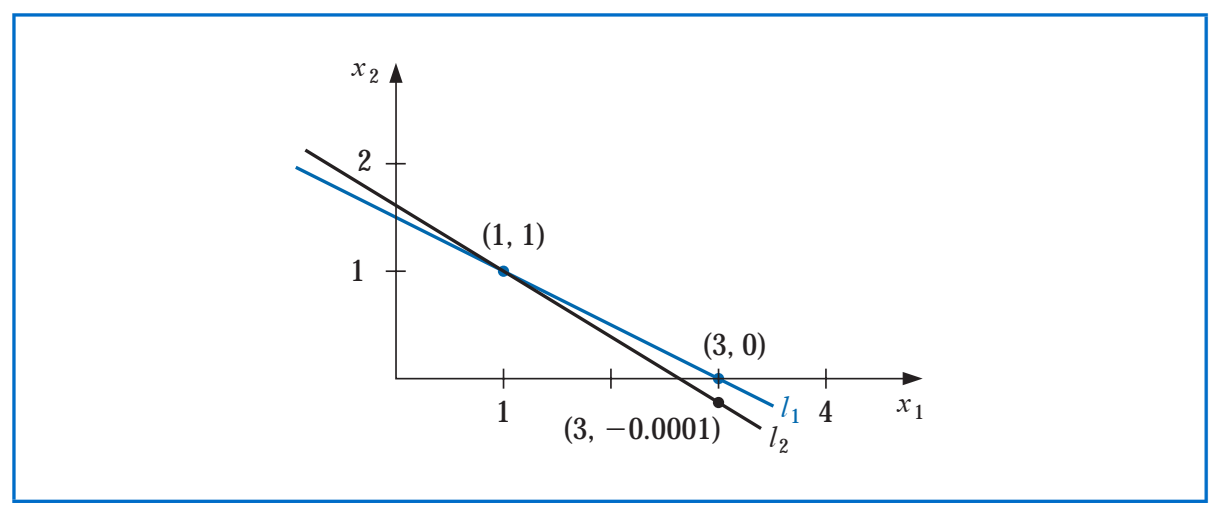
\includegraphics[width=\linewidth]{figures/figure_7.7.png}
% \caption{Minh họa cho Ví dụ 1: giao điểm của hai đường thẳng \(l_1\) và \(l_2\).}
\end{figure}

Ví dụ 1 được xây dựng có chủ đích để minh họa những khó khăn có thể xảy ra — 
và trên thực tế, thường xuyên xảy ra. 
Nếu hai đường thẳng không gần như trùng nhau, ta sẽ mong đợi rằng 
vectơ dư sẽ rất nhỏ, và khi đó nghiệm xấp xỉ sẽ chính xác.  

Trong các trường hợp tổng quát, ta không thể dựa vào hình học của hệ 
để suy ra khi nào vấn đề có thể xảy ra. 
Tuy nhiên, ta có thể thu được thông tin này bằng cách xét đến các chuẩn 
của ma trận \( A \) và ma trận nghịch đảo của nó.

\textbf{Định lý 7.27.}  
Giả sử \( \tilde{x} \) là nghiệm xấp xỉ của hệ \( A x = b \), 
\( A \) là ma trận khả nghịch, và \( r \) là vectơ dư tương ứng với \( \tilde{x} \).  
Khi đó, với mọi chuẩn (norm) tự nhiên, ta có:
\[
\|x - \tilde{x}\| \leq \|r\| \cdot \|A^{-1}\|,
\]
và nếu \( x \neq 0 \) và \( b \neq 0 \),
\[
\frac{\|x - \tilde{x}\|}{\|x\|} \leq \|A\| \cdot \|A^{-1}\| \cdot \frac{\|r\|}{\|b\|}.
\tag{7.20}
\]

\textbf{Chứng minh.}  
Vì \( r = b - A\tilde{x} = A x - A\tilde{x} \) và \( A \) khả nghịch, ta có
\( x - \tilde{x} = A^{-1} r \).  
Định lý 7.11 (trang 440) cho ta:
\[
\|x - \tilde{x}\| = \|A^{-1} r\| \leq \|A^{-1}\| \cdot \|r\|.
\]
Hơn nữa, vì \( b = A x \), nên \( \|b\| \leq \|A\| \cdot \|x\| \).  
Do đó \( 1/\|x\| \leq \|A\| / \|b\| \), và suy ra:
\[
\frac{\|x - \tilde{x}\|}{\|x\|} 
\leq \|A\| \cdot \|A^{-1}\| \cdot \frac{\|r\|}{\|b\|}.
\quad \blacksquare
\]

\subsection{Số điều kiện (Condition Numbers).}  
Bất đẳng thức trong Định lý 7.27 cho thấy rằng \( \|A^{-1}\| \) và \( \|A\| \)
cung cấp một chỉ số về mối quan hệ giữa vectơ dư và độ chính xác của nghiệm xấp xỉ.  
Trong thực tế, sai số tương đối 
\[
\frac{\|x - \tilde{x}\|}{\|x\|}
\]
là đại lượng được quan tâm nhiều nhất.  
Theo Bất đẳng thức (7.20), sai số tương đối này bị chặn trên bởi 
tích \( \|A\| \cdot \|A^{-1}\| \) nhân với sai số tương đối của vectơ dư, 
\[
\frac{\|r\|}{\|b\|}.
\]
Bất kỳ chuẩn thuận tiện nào cũng có thể được sử dụng cho phép xấp xỉ này, 
miễn là chuẩn đó được dùng nhất quán trong toàn bộ quá trình.

\textbf{Định nghĩa 7.28.}  
\textit{Số điều kiện (condition number)} của một ma trận khả nghịch \( A \)
tương ứng với một chuẩn \( \|\cdot\| \) được định nghĩa bởi:
\[
K(A) = \|A\| \cdot \|A^{-1}\|.
\]

Với ký hiệu này, các bất đẳng thức trong Định lý 7.27 có thể được viết lại thành:
\[
\|x - \tilde{x}\| \leq K(A) \frac{\|r\|}{\|A\|},
\]
và
\[
\frac{\|x - \tilde{x}\|}{\|x\|} \leq K(A) \frac{\|r\|}{\|b\|}.
\]

Với mọi ma trận khả nghịch \( A \) và chuẩn tự nhiên \( \|\cdot\| \), ta có:
\[
1 = \|I\| = \|A A^{-1}\| \leq \|A\| \cdot \|A^{-1}\| = K(A).
\]

Một ma trận được gọi là \textbf{điều kiện tốt} (well-conditioned) nếu \( K(A) \) gần 1, 
và là \textbf{kém điều kiện} (ill-conditioned) nếu \( K(A) \) lớn đáng kể hơn 1.  
Trong ngữ cảnh này, “độ điều kiện” phản ánh mức độ tin cậy rằng 
một vectơ dư nhỏ sẽ tương ứng với một nghiệm xấp xỉ đủ chính xác.

\textbf{Ví dụ 2.}  
Xác định số điều kiện của ma trận
\[
A = 
\begin{bmatrix}
1 & 2 \\
1.0001 & 2
\end{bmatrix}.
\]

\textbf{Lời giải.}  
Trong Ví dụ 1, ta thấy rằng nghiệm xấp xỉ \( (3, -0.0001)^T \) của nghiệm chính xác \( (1, 1)^T \) 
cho một vectơ dư rất nhỏ. Điều này cho thấy số điều kiện của \( A \) phải lớn.  
Ta có \( \|A\|_{\infty} = \max(|1| + |2|, |1.0001| + |2|) = 3.0001 \), 
và đây không phải là một giá trị lớn. Tuy nhiên,
\[
A^{-1} =
\begin{bmatrix}
-10000 & 10000 \\
5000.5 & -5000
\end{bmatrix},
\]
nên \( \|A^{-1}\|_{\infty} = 20000 \).  
Vì vậy, đối với chuẩn vô cực, ta có
\[
K(A) = (20000)(3.0001) = 60002.
\]
Kích thước của số điều kiện trong ví dụ này đủ lớn để cảnh báo rằng 
ta không nên đánh giá cao tính chính xác của nghiệm chỉ dựa trên độ nhỏ của vectơ dư.

Số điều kiện \( K_{\infty} \) có thể được tính trong Maple 
bằng cách sử dụng gói \texttt{LinearAlgebra} và ma trận \( A \).  
Khi đó, lệnh \texttt{ConditionNumber(A)} sẽ cho số điều kiện trong chuẩn \( l_{\infty} \).  
Ví dụ, ta có thể tính số điều kiện của ma trận \( A \) trong Ví dụ 2 bằng:
\[
A := \texttt{Matrix([[1,2],[1.0001,2]]): \ ConditionNumber(A)}
\]
và kết quả là
\[
60002.00000.
\]

Mặc dù số điều kiện của ma trận phụ thuộc hoàn toàn vào các chuẩn của ma trận và của nghịch đảo của nó, 
việc tính toán nghịch đảo chịu ảnh hưởng bởi sai số làm tròn và phụ thuộc vào độ chính xác của số học được sử dụng.  
Nếu các phép tính chỉ được thực hiện với \( t \) chữ số chính xác, 
số điều kiện xấp xỉ của ma trận \( A \) là chuẩn của \( A \) nhân với chuẩn của nghịch đảo xấp xỉ của \( A \), 
được tính bằng số học \( t \)-chữ số.  
Trên thực tế, số điều kiện cũng phụ thuộc vào phương pháp được dùng để tính nghịch đảo.  
Vì số lượng phép toán cần thiết để tính nghịch đảo có thể lớn, 
ta thường cần ước lượng số điều kiện mà không cần tính trực tiếp nghịch đảo.

Nếu ta giả sử rằng nghiệm xấp xỉ của hệ tuyến tính \( A x = b \) 
được tính bằng số học \( t \)-chữ số và phép khử Gauss, 
thì (theo [FM], trang 45–47) có thể chứng minh rằng vectơ dư \( r \) cho nghiệm xấp xỉ \( \tilde{x} \) thỏa mãn
\[
\|r\| \approx 10^{-t} \|A\| \cdot \|\tilde{x}\|.
\tag{7.21}
\]

Từ xấp xỉ này, ta có thể ước lượng \textit{số điều kiện hiệu dụng} (effective condition number) 
trong phép tính số học \( t \)-chữ số mà không cần phải tính nghịch đảo của ma trận \( A \).  
Thực tế, xấp xỉ này giả định rằng tất cả các phép toán số học trong quá trình khử Gauss 
được thực hiện bằng số học \( t \)-chữ số, 
nhưng các phép toán cần thiết để xác định vectơ dư được thực hiện bằng số học hai lần chính xác 
(tức là \( 2t \)-chữ số).  
Kỹ thuật này không làm tăng đáng kể chi phí tính toán, 
nhưng loại bỏ đáng kể mất mát độ chính xác xảy ra do việc trừ các số gần bằng nhau 
trong quá trình tính vectơ dư.

Xấp xỉ cho số điều kiện trong số học \( t \)-chữ số, ký hiệu \( K(A) \), 
có thể được rút ra từ việc xét hệ tuyến tính
\[
A y = r.
\]
Nghiệm của hệ này có thể được xấp xỉ dễ dàng, 
vì các hệ số nhân (multipliers) trong phép khử Gauss đã được tính sẵn.  
Vì vậy, ta có thể phân tích \( A \) dưới dạng \( P^T L U \) như trong Mục 5 của Chương 6.  
Trên thực tế, nghiệm xấp xỉ của hệ \( A y = r \) thỏa
\[
\tilde{y} \approx A^{-1} r = A^{-1}(b - A\tilde{x}) = A^{-1}b - A^{-1}A\tilde{x} = x - \tilde{x},
\tag{7.22}
\]
và
\[
x \approx \tilde{x} + \tilde{y}.
\]
Do đó, \( \tilde{y} \) là ước lượng cho sai số khi \( \tilde{x} \) xấp xỉ nghiệm chính xác \( x \) của hệ \( A x = b \).  
Từ các biểu thức (7.21) và (7.22), ta có:
\[
\|\tilde{y}\| \approx \|x - \tilde{x}\| \approx \|A^{-1} r\| 
\leq \|A^{-1}\| \cdot \|r\| 
\approx \|A^{-1}\| \cdot \|A\| \cdot 10^{-t} \|\tilde{x}\| 
= 10^{-t} \|\tilde{x}\| K(A).
\]

Điều này cho ta một xấp xỉ cho số điều kiện liên quan đến việc giải hệ \( A x = b \)
bằng phép khử Gauss và số học \( t \)-chữ số:
\[
K(A) \approx \frac{\|\tilde{y}\|}{\|\tilde{x}\|} \, 10^{t}.
\tag{7.23}
\]

\textbf{Minh họa.}  
Hệ tuyến tính được cho bởi
\[
\begin{bmatrix}
3.3330 & 15920 & -10.333 \\
2.2220 & 16.710 & 9.6120 \\
1.5611 & 5.1791 & 1.6852
\end{bmatrix}
\begin{bmatrix}
x_1 \\ x_2 \\ x_3
\end{bmatrix}
=
\begin{bmatrix}
15913 \\ 28.544 \\ 8.4254
\end{bmatrix}
\]
có nghiệm chính xác là \( x = (1, 1, 1)^T \).

Sử dụng phép khử Gauss với làm tròn 5 chữ số, 
ta nhận được các ma trận mở rộng:
\[
\begin{bmatrix}
3.3330 & 15920 & -10.333 & 15913 \\
0 & -10596 & 16.501 & 10580 \\
0 & -7451.4 & 6.5250 & -7444.9
\end{bmatrix}
\]
và
\[
\begin{bmatrix}
3.3330 & 15920 & -10.333 & 15913 \\
0 & -10596 & 16.501 & -10580 \\
0 & 0 & -5.0790 & -4.7000
\end{bmatrix}.
\]

Nghiệm xấp xỉ của hệ này là
\[
\tilde{x} = (1.2001,\ 0.99991,\ 0.92538)^T.
\]

Vector dư tương ứng với $\bar{x}$ được tính bằng độ chính xác kép như sau:

\[
\mathbf{r} = \mathbf{b} - A\bar{x}
\]

\[
=
\begin{bmatrix}
15913 \\[3pt]
28.544 \\[3pt]
8.4254
\end{bmatrix}
-
\begin{bmatrix}
3.3330 & 15920 & -10.333 \\[3pt]
2.2220 & 16.710 & 9.6120 \\[3pt]
1.5611 & 5.1791 & 1.6852
\end{bmatrix}
\begin{bmatrix}
1.2001 \\[3pt]
0.99991 \\[3pt]
0.92538
\end{bmatrix}
\]

\[
=
\begin{bmatrix}
15913 \\[3pt]
28.544 \\[3pt]
8.4254
\end{bmatrix}
-
\begin{bmatrix}
15913.00518 \\[3pt]
28.26987086 \\[3pt]
8.611560367
\end{bmatrix}
=
\begin{bmatrix}
-0.00518 \\[3pt]
0.27412914 \\[3pt]
-0.186160367
\end{bmatrix},
\]

do đó

\[
\|\mathbf{r}\|_\infty = 0.27413.
\]

Ước lượng cho số điều kiện được cho trong phần thảo luận trước đó được xác định bằng cách đầu tiên giải hệ $A y = r$ để tìm $\bar{y}$:

\[
\begin{bmatrix}
3.3330 & 15920 & -10.333 \\[3pt]
2.2220 & 16.710 & 9.6120 \\[3pt]
1.5611 & 5.1791 & 1.6852
\end{bmatrix}
\begin{bmatrix}
y_1 \\[3pt] y_2 \\[3pt] y_3
\end{bmatrix}
=
\begin{bmatrix}
-0.00518 \\[3pt]
0.27413 \\[3pt]
-0.18616
\end{bmatrix}.
\]

Điều này cho ta:

\[
\bar{y} = (-0.20008,\; 8.9987 \times 10^{-5},\; -0.0744607)^{T}.
\]

Sử dụng ước lượng trong phương trình (7.23) ta có:

\[
K(A) \approx \frac{\|\bar{y}\|_\infty}{\|\bar{x}\|_\infty} \times 10^{5} = \frac{0.20008}{1.2001} \times 10^{5} = 16672. \tag{7.24}
\]

Để xác định chính xác số điều kiện của $A$, trước hết ta phải tìm $A^{-1}$.  
Sử dụng số học làm tròn trong quá trình tính toán, ta có xấp xỉ sau:

\[
A^{-1} \approx
\begin{bmatrix}
-1.1701 \times 10^{-4} & -1.4983 \times 10^{-1} & 8.5416 \times 10^{-1} \\[3pt]
6.2782 \times 10^{-5} & 1.2124 \times 10^{-4} & -3.0662 \times 10^{-4} \\[3pt]
-8.6631 \times 10^{-5} & 1.3846 \times 10^{-1} & -1.9689 \times 10^{-1}
\end{bmatrix}.
\]

Định lý 7.11 ở trang 440 cho biết rằng $\|A^{-1}\|_\infty = 1.0041$ và $\|A\|_\infty = 15934$.  
Do đó, ma trận $A$ có điều kiện kém này có:

\[
K(A) = (1.0041)(15934) = 15999.
\]

Ước lượng trong (7.24) khá gần với giá trị chính xác của $K(A)$ và yêu cầu ít công sức tính toán hơn đáng kể.

Vì nghiệm thực sự là $x = (1, 1, 1)^{T}$ đã biết cho hệ này, ta có thể tính được rằng

\[
\|\mathbf{x} - \bar{\mathbf{x}}\|_\infty = 0.2001
\quad \text{và} \quad
\frac{\|\mathbf{x} - \bar{\mathbf{x}}\|_\infty}{\|\mathbf{x}\|_\infty}
= \frac{0.2001}{1} = 0.2001.
\]

Các giới hạn sai số được nêu trong Định lý 7.27 cho các giá trị này là

\[
\frac{\|\mathbf{x} - \bar{\mathbf{x}}\|_\infty}{\|\mathbf{x}\|_\infty}
\leq K(A) \frac{\|\mathbf{r}\|_\infty}{\|A\|_\infty}
= \frac{(15999)(0.27413)}{15934} = 0.27525
\]

và

\[
\frac{\|\mathbf{x} - \bar{\mathbf{x}}\|_\infty}{\|\mathbf{x}\|_\infty}
\leq K(A) \frac{\|\mathbf{r}\|_\infty}{\|\mathbf{b}\|_\infty}
= \frac{(15999)(0.27413)}{15913} = 0.27561.
\]

\subsection{Tinh chỉnh lặp (Iterative Refinement)}

Trong Phương trình (7.22), ta đã sử dụng ước lượng $\bar{y} \approx \mathbf{x} - \bar{\mathbf{x}}$, trong đó $\bar{y}$ là nghiệm xấp xỉ của hệ tuyến tính $A y = \mathbf{r}$.  
Nói chung, $\bar{\mathbf{x}} + \bar{y}$ là một xấp xỉ chính xác hơn cho nghiệm của hệ tuyến tính $A \mathbf{x} = \mathbf{b}$ so với xấp xỉ ban đầu $\bar{\mathbf{x}}$.  
Phương pháp sử dụng giả định này được gọi là \textit{tinh chỉnh lặp} (\textit{iterative refinement}) hay \textit{cải thiện lặp} (\textit{iterative improvement}), và bao gồm việc thực hiện nhiều phép lặp trên hệ có vế phải là vector dư, để có được các xấp xỉ liên tiếp cho đến khi đạt được kết quả có độ chính xác thỏa đáng.

Nếu quá trình này được áp dụng bằng số học có $t$ chữ số và nếu $K_{\infty}(A) \approx 10^{q}$, thì sau $k$ vòng lặp tinh chỉnh lặp, nghiệm thu được sẽ có xấp xỉ bằng số chữ số nhỏ hơn giữa $t$ và $t(k - q)$ chữ số chính xác.  
Nếu hệ có điều kiện tốt, một hoặc hai lần lặp thường đủ để xác nhận rằng nghiệm là chính xác.  
Có khả năng cải thiện đáng kể trên các hệ có điều kiện kém, trừ khi ma trận $A$ có điều kiện quá tệ đến mức $K_{\infty}(A) > 10^{t}$.  
Trong tình huống đó, nên sử dụng độ chính xác cao hơn cho các phép tính.

\subsection*{Thuật toán 7.4 — Tinh chỉnh lặp (Iterative Refinement)}

\textbf{Mục tiêu:}  
Xấp xỉ nghiệm cho hệ tuyến tính $A\mathbf{x} = \mathbf{b}$.

\textbf{Dữ liệu đầu vào:}
\begin{itemize}
    \item Số lượng phương trình và ẩn $n$;
    \item Các phần tử $a_{ij},\; 1 \leq i, j \leq n$ của ma trận $A$;
    \item Các phần tử $b_i,\; 1 \leq i \leq n$ của $\mathbf{b}$;
    \item Số lần lặp tối đa $N$;
    \item Ngưỡng sai số $TOL$;
    \item Số chữ số chính xác $t$.
\end{itemize}

\textbf{Dữ liệu đầu ra:}  
Nghiệm xấp xỉ $\mathbf{x} = (x_1, x_2, \dots, x_n)^{T}$ hoặc thông báo rằng số lần lặp vượt quá giới hạn, kèm theo giá trị xấp xỉ của số điều kiện $\text{COND} \approx K_{\infty}(A)$.


Giải hệ $A\mathbf{x} = \mathbf{b}$ cho $x_1, \dots, x_n$ bằng phương pháp khử Gauss, lưu các hệ số nhân $m_{ij},\; j = i+1, i+2, \dots, n;\; i = 1, 2, \dots, n-1$ và lưu lại các phép hoán đổi hàng.

\begin{enumerate}[label=\textbf{Step \arabic*:}, leftmargin=2.5em]

\item Đặt $k = 1$.

\item Trong khi $(k \leq N)$ thì thực hiện các Bước 3–9.

\item Với $i = 1, 2, \dots, n$ (tính $\mathbf{r}$):
\[
r_i = b_i - \sum_{j=1}^{n} a_{ij}x_j.
\]
(Thực hiện các phép tính bằng số học độ chính xác kép.)

\item Giải hệ tuyến tính $A y = \mathbf{r}$ bằng phương pháp khử Gauss theo cùng thứ tự như ở Bước 0.

\item Với $i = 1, \dots, n$, đặt $x_i := x_i + y_i$.

\item Nếu $k = 1$ thì đặt 
\[
\text{COND} = \frac{\|\mathbf{y}\|_{\infty}}{\|\mathbf{x}\|_{\infty}} \times 10^{t}.
\]

\item Nếu $\|\mathbf{x} - \bar{\mathbf{x}}\|_{\infty} < TOL$ thì  
\textbf{OUTPUT} $(\mathbf{x})$;  
\textbf{OUTPUT} $(\text{COND});$  
\textbf{(Thuật toán đã hội tụ thành công.)}  
\textbf{STOP.}

\item Đặt $k = k + 1$.

\item Với $i = 1, \dots, n$, đặt $x_i := x_i$.

\item OUTPUT (‘Số lần lặp tối đa đã bị vượt quá’); \\
OUTPUT (COND); \\
\textit{(Thuật toán không thành công.)} \\
STOP.

\end{enumerate}


Nếu sử dụng số học $t$-chữ số, một quy tắc dừng được khuyến nghị trong Bước 7 là lặp lại cho đến khi
\[
|y_i^{(k)}| \leq 10^{-t}, \quad \text{với mỗi } i = 1, 2, \dots, n.
\]

\subsection*{Minh họa}

Trong ví dụ trước, ta đã tìm được nghiệm xấp xỉ cho hệ tuyến tính
\[
\begin{bmatrix}
3.3330 & 15920 & -10.333 \\[3pt]
2.2220 & 16.710 & 9.6120 \\[3pt]
1.5611 & 5.1791 & 1.6852
\end{bmatrix}
\begin{bmatrix}
x_1 \\[3pt]
x_2 \\[3pt]
x_3
\end{bmatrix}
=
\begin{bmatrix}
15913 \\[3pt]
28.544 \\[3pt]
8.4254
\end{bmatrix}
\]
bằng cách sử dụng số học 5 chữ số và khử Gauss, thu được
\[
\bar{\mathbf{x}}^{(1)} = (1.2001,\, 0.99991,\, 0.92538)^{T}.
\]

Nghiệm của hệ $A y = \mathbf{r}^{(1)}$ được tính là
\[
\bar{\mathbf{y}}^{(1)} = (-0.20008,\, 8.9987 \times 10^{-5},\, -0.0744607)^{T}.
\]

Theo Bước 5 của thuật toán này, ta có
\[
\bar{\mathbf{x}}^{(2)} = \bar{\mathbf{x}}^{(1)} + \bar{\mathbf{y}}^{(1)} = (1.0000,\, 1.00000,\, 0.99999)^{T}.
\]

Sai số thực tế trong xấp xỉ này là
\[
\|\mathbf{x} - \bar{\mathbf{x}}^{(2)}\|_{\infty} = 1 \times 10^{-5}.
\]

Sử dụng quy tắc dừng được đề xuất cho thuật toán, ta tính
\[
\mathbf{r}^{(2)} = \mathbf{b} - A \bar{\mathbf{x}}^{(2)},
\]
và giải hệ $A y^{(2)} = \mathbf{r}^{(2)}$, thu được
\[
\bar{\mathbf{y}}^{(2)} = (1.5002 \times 10^{-9},\, 2.0951 \times 10^{-10},\, -1.0000 \times 10^{-5})^{T}.
\]

Vì $\|\bar{\mathbf{y}}^{(2)}\|_{\infty} \leq 10^{-5}$, ta kết luận rằng
\[
\bar{\mathbf{x}}^{(3)} = \bar{\mathbf{x}}^{(2)} + \bar{\mathbf{y}}^{(2)} = (1.0000,\, 1.0000,\, 1.0000)^{T}
\]
là nghiệm đủ chính xác — và điều đó hoàn toàn đúng.

\vspace{0.5em}

Trong toàn bộ phần này, ta đã giả định rằng trong hệ tuyến tính $A\mathbf{x} = \mathbf{b}$, cả $A$ và $\mathbf{b}$ đều được biểu diễn chính xác.  
Trên thực tế, các phần tử $a_{ij}$ và $b_j$ có thể bị thay đổi hoặc nhiễu đi một lượng nhỏ $\delta a_{ij}$ và $\delta b_j$, khiến cho hệ tuyến tính trở thành:

\[
(A + \delta A)\mathbf{x} = \mathbf{b} + \delta \mathbf{b}.
\]

Hệ này được giải để tìm $\mathbf{x}$ trong phương trình $A\mathbf{x} = \mathbf{b}$.  
Thông thường, nếu $\|\delta A\|$ và $\|\delta \mathbf{b}\|$ đều nhỏ (cỡ $10^{-t}$), thì số học $t$-chữ số sẽ cho ra một nghiệm $\bar{\mathbf{x}}$ mà sai số $\|\mathbf{x} - \bar{\mathbf{x}}\|$ cũng tương ứng nhỏ.  
Tuy nhiên, trong trường hợp các hệ có điều kiện kém, ta đã thấy rằng ngay cả khi $A$ và $\mathbf{b}$ được biểu diễn chính xác, các lỗi làm tròn cũng có thể khiến $\|\mathbf{x} - \bar{\mathbf{x}}\|$ trở nên lớn. Định lý tiếp theo liên hệ sự nhiễu loạn (sai lệch) của các hệ phương trình tuyến tính với số điều kiện (condition number) của một ma trận. Chứng minh của kết quả này có thể được tìm thấy trong [Or2], trang 33.


\subsection*{Định lý 7.29}

Giả sử \(A\) là khả nghịch và
\[
\|\delta A\| < \frac{1}{\|A^{-1}\|}.
\]

Nghiệm \(\tilde{x}\) của hệ
\[
(A + \delta A)\tilde{x} = \mathbf{b} + \delta\mathbf{b}
\]
xấp xỉ nghiệm \(\mathbf{x}\) của \(A\mathbf{x} = \mathbf{b}\) với ước lượng sai số

\[
\frac{\|\mathbf{x} - \tilde{\mathbf{x}}\|}{\|\mathbf{x}\|}
\le
\frac{K(A)\,\|A\|}{\|A\| - K(A)\|\delta A\|}
\left(
\frac{\|\delta\mathbf{b}\|}{\|\mathbf{b}\|}
+
\frac{\|\delta A\|}{\|A\|}
\right).
\tag{7.25}
\]

Ước lượng trong bất đẳng thức (7.25) phát biểu rằng nếu ma trận \(A\) có điều kiện tốt (tức là \(K(A)\) không quá lớn), thì các thay đổi nhỏ trong \(A\) và \(\mathbf{b}\) sẽ tạo ra những thay đổi tương ứng nhỏ trong nghiệm \(\mathbf{x}\). Ngược lại, nếu \(A\) có điều kiện kém, thì những thay đổi nhỏ trong \(A\) và \(\mathbf{b}\) có thể gây ra thay đổi lớn trong \(\mathbf{x}\).

Định lý này không phụ thuộc vào phương pháp số cụ thể được dùng để giải \(A\mathbf{x} = \mathbf{b}\).  
Người ta có thể chứng minh, bằng phân tích sai số ngược (backward error analysis), rằng nếu khử Gauss có pivot được sử dụng để giải \(A\mathbf{x} = \mathbf{b}\) trong số học có \(t\) chữ số, thì nghiệm số \(\tilde{\mathbf{x}}\) là nghiệm thực của một hệ tuyến tính dạng:

\[
(A + \delta A)\tilde{\mathbf{x}} = \mathbf{b},
\qquad\text{trong đó}\quad
\|\delta A\|_\infty \le f(n)10^{1-t}\max_{i,j,k}|a_{ij}^{(k)}|,
\]

với một hàm số \(f(n)\). Wilkinson nhận thấy rằng trong thực tế \(f(n)\approx n\) và, trong trường hợp xấu nhất, \(f(n) \le 1.01(n^3 + 3n^2)\).


